% !TeX spellcheck = hu_HU
% !TeX encoding = UTF-8
% !TeX program = xelatex
% TODO Change language to en_GB (recommended) or en_US for English documents
\documentclass[11pt,a4paper,oneside]{report}             % Single-side
%\documentclass[11pt,a4paper,twoside,openright]{report}  % Duplex

% thanks to http://tex.stackexchange.com/a/47579/71109
\usepackage{ifxetex}
\usepackage{ifluatex}
\newif\ifxetexorluatex % a new conditional starts as false
\ifnum 0\ifxetex 1\fi\ifluatex 1\fi>0
   \xetexorluatextrue
\fi

\ifxetexorluatex
  \usepackage{fontspec}
\else
  \usepackage[T1]{fontenc}
  \usepackage[utf8]{inputenc}
  \usepackage[lighttt]{lmodern}
\fi

\usepackage[english,magyar]{babel} % Alapértelmezés szerint utoljára definiált nyelv lesz aktív, de később külön beállítjuk az aktív nyelvet.

%\usepackage{cmap}
\usepackage{amsfonts,amsmath,amssymb} % Mathematical symbols.
%\usepackage[ruled,boxed,resetcount,linesnumbered]{algorithm2e} % For pseudocodes. % beware: this is not compatible with LuaLaTeX, see http://tex.stackexchange.com/questions/34814/lualatex-and-algorithm2e
\usepackage{booktabs} % For publication quality tables for LaTeX
\usepackage{graphicx}

%\usepackage{fancyhdr}
%\usepackage{lastpage}

\usepackage{anysize}
%\usepackage{sectsty}
\usepackage{setspace} % For setting line spacing

\usepackage[unicode]{hyperref} % For hyperlinks in the generated document.
\usepackage{xcolor}
\usepackage{listings} % For source code snippets.

\usepackage[amsmath,thmmarks]{ntheorem} % Theorem-like environments.

\usepackage[hang]{caption}

\singlespacing

\newcommand{\selecthungarian}{
	\selectlanguage{magyar}
	\setlength{\parindent}{2em}
	\setlength{\parskip}{0em}
	\frenchspacing
}

\newcommand{\selectenglish}{
	\selectlanguage{english}
	\setlength{\parindent}{0em}
	\setlength{\parskip}{0.5em}
	\nonfrenchspacing
	\renewcommand{\figureautorefname}{Figure}
	\renewcommand{\tableautorefname}{Table}
	\renewcommand{\partautorefname}{Part}
	\renewcommand{\chapterautorefname}{Chapter}
	\renewcommand{\sectionautorefname}{Section}
	\renewcommand{\subsectionautorefname}{Section}
	\renewcommand{\subsubsectionautorefname}{Section}
}

\usepackage[numbers]{natbib}
\usepackage{xspace}

\usepackage{pdfpages}

\usepackage{subcaption}
\captionsetup{compatibility=false}

\usepackage{algorithm}
\usepackage{algpseudocode}
\usepackage{amsmath}

\usepackage{setspace}

%TODO Set the main variables
\newcommand{\vikszerzoVezeteknev}{Bálint}
\newcommand{\vikszerzoKeresztnev}{Gergő}

\newcommand{\vikkonzulensBMegszolitas}{Dr.~}
\newcommand{\vikkonzulensBVezeteknev}{Szűcs}
\newcommand{\vikkonzulensBKeresztnev}{Gábor}

\newcommand{\vikkonzulensAMegszolitas}{}
\newcommand{\vikkonzulensAVezeteknev}{Kiss}
\newcommand{\vikkonzulensAKeresztnev}{Richárd}

\newcommand{\vikkonzulensCMegszolitas}{}
\newcommand{\vikkonzulensCVezeteknev}{}
\newcommand{\vikkonzulensCKeresztnev}{}

\newcommand{\vikcim}{Investigating graph-based representation learning and developing a new inductive method} % Cím
\newcommand{\viktanszek}{\bmemit} % Tanszék
\newcommand{\vikdoktipus}{\msc} % Dokumentum típusa (\bsc vagy \msc)
\newcommand{\vikmunkatipusat}{diplomatervet} % a "hallgató nyilatkozat" részhez: szakdolgozatot vagy diplomatervet

\newcommand{\szerzoMeta}{\vikszerzoVezeteknev{} \vikszerzoKeresztnev} % egy szerző esetén
%\newcommand{\szerzoMeta}{\vikszerzoVezeteknev{} \vikszerzoKeresztnev, \tdkszerzoB} % két szerző esetén

%TODO Language configuration -- choose one
% Beállítások magyar nyelvű dolgozathoz
%%--------------------------------------------------------------------------------------
% Elnevezések
%--------------------------------------------------------------------------------------
\newcommand{\bme}{Budapesti Műszaki és Gazdaságtudományi Egyetem}
\newcommand{\vik}{Villamosmérnöki és Informatikai Kar}

\newcommand{\bmemit}{Távközlési és Médiainformatikai Tanszék}

\newcommand{\keszitette}{Készítette}
\newcommand{\konzulens}{Konzulens}

\newcommand{\bsc}{Szakdolgozat}
\newcommand{\msc}{Diplomaterv}
\newcommand{\tdk}{TDK dolgozat}
\newcommand{\bsconlab}{BSc Önálló laboratórium}
\newcommand{\msconlabi}{MSc Önálló laboratórium 1.}
\newcommand{\msconlabii}{MSc Önálló laboratórium 2.}

\newcommand{\pelda}{Példa}
\newcommand{\definicio}{Definíció}
\newcommand{\tetel}{Tétel}

\newcommand{\bevezetes}{Bevezetés}
\newcommand{\koszonetnyilvanitas}{Köszönetnyilvánítás}
\newcommand{\fuggelek}{Függelék}

% Opcionálisan átnevezhető címek
%\addto\captionsmagyar{%
%\renewcommand{\listfigurename}{Saját ábrajegyzék cím}
%\renewcommand{\listtablename}{Saját táblázatjegyzék cím}
%\renewcommand{\bibname}{Saját irodalomjegyzék név}
%}

\newcommand{\szerzo}{\vikszerzoVezeteknev{} \vikszerzoKeresztnev}
\newcommand{\vikkonzulensA}{\vikkonzulensAMegszolitas\vikkonzulensAVezeteknev{} \vikkonzulensAKeresztnev}
\newcommand{\vikkonzulensB}{\vikkonzulensBMegszolitas\vikkonzulensBVezeteknev{} \vikkonzulensBKeresztnev}
\newcommand{\vikkonzulensC}{\vikkonzulensCMegszolitas\vikkonzulensCVezeteknev{} \vikkonzulensCKeresztnev}

\newcommand{\selectthesislanguage}{\selecthungarian}

\bibliographystyle{huplain}

\def\lstlistingname{lista}

\newcommand{\appendixnumber}{6}  % a fofejezet-szamlalo az angol ABC 6. betuje (F) lesz

% Settings for English documents
%--------------------------------------------------------------------------------------
% Elnevezések
%--------------------------------------------------------------------------------------
\newcommand{\bme}{Budapest University of Technology and Economics}
\newcommand{\vik}{Faculty of Electrical Engineering and Informatics}

\newcommand{\bmemit}{Department of Measurement and Information Systems}

\newcommand{\keszitette}{Author}
\newcommand{\konzulens}{Advisor}

\newcommand{\bsc}{Bachelor's Thesis}
\newcommand{\msc}{Master's Thesis}
\newcommand{\tdk}{Scientific Students' Association Report}
\newcommand{\bsconlab}{BSc Project Laboratory}
\newcommand{\msconlabi}{MSc Project Laboratory 1}
\newcommand{\msconlabii}{MSc Project Laboratory 2}

\newcommand{\pelda}{Example}
\newcommand{\definicio}{Definition}
\newcommand{\tetel}{Theorem}

\newcommand{\bevezetes}{Introduction}
\newcommand{\koszonetnyilvanitas}{Acknowledgements}
\newcommand{\fuggelek}{Appendix}

% Optional custom titles
%\addto\captionsenglish{%
%\renewcommand*{\listfigurename}{Your list of figures title}
%\renewcommand*{\listtablename}{Your list of tables title}
%\renewcommand*{\bibname}{Your bibliography title}
%}

\newcommand{\szerzo}{\vikszerzoKeresztnev{} \vikszerzoVezeteknev}
\newcommand{\vikkonzulensA}{\vikkonzulensAMegszolitas\vikkonzulensAKeresztnev{} \vikkonzulensAVezeteknev}
\newcommand{\vikkonzulensB}{\vikkonzulensBMegszolitas\vikkonzulensBKeresztnev{} \vikkonzulensBVezeteknev}
\newcommand{\vikkonzulensC}{\vikkonzulensCMegszolitas\vikkonzulensCKeresztnev{} \vikkonzulensCVezeteknev}

\newcommand{\selectthesislanguage}{\selectenglish}

\bibliographystyle{plainnat}

\newcommand{\ie}{i.e.\@\xspace}
\newcommand{\Ie}{I.e.\@\xspace}
\newcommand{\eg}{e.g.\@\xspace}
\newcommand{\Eg}{E.g.\@\xspace}
\newcommand{\etal}{et al.\@\xspace}
\newcommand{\etc}{etc.\@\xspace}
\newcommand{\vs}{vs.\@\xspace}
\newcommand{\viz}{viz.\@\xspace} % videlicet
\newcommand{\cf}{cf.\@\xspace} % confer
\newcommand{\Cf}{Cf.\@\xspace}
\newcommand{\wrt}{w.r.t.\@\xspace} % with respect to
\newcommand{\approximately}{approx.\@\xspace}

\newcommand{\appendixnumber}{1}  % a fofejezet-szamlalo az angol ABC 1. betuje (A) lesz


%--------------------------------------------------------------------------------------
% Page layout setup
%--------------------------------------------------------------------------------------
% we need to redefine the pagestyle plain
% another possibility is to use the body of this command without \fancypagestyle
% and use \pagestyle{fancy} but in that case the special pages
% (like the ToC, the References, and the Chapter pages)remain in plane style

\pagestyle{plain}
\marginsize{35mm}{25mm}{15mm}{15mm}

\setcounter{tocdepth}{3}
%\sectionfont{\large\upshape\bfseries}
\setcounter{secnumdepth}{3}

\sloppy % Margón túllógó sorok tiltása.
\widowpenalty=10000 \clubpenalty=10000 %A fattyú- és árvasorok elkerülése
\def\hyph{-\penalty0\hskip0pt\relax} % Kötőjeles szavak elválasztásának engedélyezése


%--------------------------------------------------------------------------------------
% Setup hyperref package
%--------------------------------------------------------------------------------------
\hypersetup{
    % bookmarks=true,            % show bookmarks bar?
    unicode=true,              % non-Latin characters in Acrobat's bookmarks
    pdftitle={\vikcim},        % title
    pdfauthor={\szerzoMeta},    % author
    pdfsubject={\vikdoktipus}, % subject of the document
    pdfcreator={\szerzoMeta},   % creator of the document
    pdfproducer={},    % producer of the document
    pdfkeywords={},    % list of keywords (separate then by comma)
    pdfnewwindow=true,         % links in new window
    colorlinks=true,           % false: boxed links; true: colored links
    linkcolor=black,           % color of internal links
    citecolor=black,           % color of links to bibliography
    filecolor=black,           % color of file links
    urlcolor=black             % color of external links
}


%--------------------------------------------------------------------------------------
% Set up listings
%--------------------------------------------------------------------------------------
\definecolor{lightgray}{rgb}{0.95,0.95,0.95}
\lstset{
	basicstyle=\scriptsize\ttfamily, % print whole listing small
	keywordstyle=\color{black}\bfseries, % bold black keywords
	identifierstyle=, % nothing happens
	% default behavior: comments in italic, to change use
	% commentstyle=\color{green}, % for e.g. green comments
	stringstyle=\scriptsize,
	showstringspaces=false, % no special string spaces
	aboveskip=3pt,
	belowskip=3pt,
	backgroundcolor=\color{lightgray},
	columns=flexible,
	keepspaces=true,
	escapeinside={(*@}{@*)},
	captionpos=b,
	breaklines=true,
	frame=single,
	float=!ht,
	tabsize=2,
	literate=*
		{á}{{\'a}}1	{é}{{\'e}}1	{í}{{\'i}}1	{ó}{{\'o}}1	{ö}{{\"o}}1	{ő}{{\H{o}}}1	{ú}{{\'u}}1	{ü}{{\"u}}1	{ű}{{\H{u}}}1
		{Á}{{\'A}}1	{É}{{\'E}}1	{Í}{{\'I}}1	{Ó}{{\'O}}1	{Ö}{{\"O}}1	{Ő}{{\H{O}}}1	{Ú}{{\'U}}1	{Ü}{{\"U}}1	{Ű}{{\H{U}}}1
}


%--------------------------------------------------------------------------------------
% Set up theorem-like environments
%--------------------------------------------------------------------------------------
% Using ntheorem package -- see http://www.math.washington.edu/tex-archive/macros/latex/contrib/ntheorem/ntheorem.pdf

\theoremstyle{plain}
\theoremseparator{.}
\newtheorem{example}{\pelda}

\theoremseparator{.}
%\theoremprework{\bigskip\hrule\medskip}
%\theorempostwork{\hrule\bigskip}
\theorembodyfont{\upshape}
\theoremsymbol{{\large \ensuremath{\centerdot}}}
\newtheorem{definition}{\definicio}

\theoremseparator{.}
%\theoremprework{\bigskip\hrule\medskip}
%\theorempostwork{\hrule\bigskip}
\newtheorem{theorem}{\tetel}


%--------------------------------------------------------------------------------------
% Some new commands and declarations
%--------------------------------------------------------------------------------------
\newcommand{\code}[1]{{\upshape\ttfamily\scriptsize\indent #1}}
\newcommand{\doi}[1]{DOI: \href{http://dx.doi.org/\detokenize{#1}}{\raggedright{\texttt{\detokenize{#1}}}}} % A hivatkozások közt így könnyebb DOI-t megadni.

\DeclareMathOperator*{\argmax}{arg\,max}
%\DeclareMathOperator*[1]{\floor}{arg\,max}
\DeclareMathOperator{\sign}{sgn}
\DeclareMathOperator{\rot}{rot}


%--------------------------------------------------------------------------------------
% Setup captions
%--------------------------------------------------------------------------------------
\captionsetup[figure]{
	width=.75\textwidth,
	aboveskip=10pt}

\renewcommand{\captionlabelfont}{\bf}
%\renewcommand{\captionfont}{\footnotesize\it}

%--------------------------------------------------------------------------------------
% Hyphenation exceptions
%--------------------------------------------------------------------------------------
\hyphenation{Shakes-peare Mar-seilles ár-víz-tű-rő tü-kör-fú-ró-gép}


\author{\vikszerzo}
\title{\viktitle}

%--------------------------------------------------------------------------------------
% Table of contents and the main text
%--------------------------------------------------------------------------------------
\begin{document}

\pagenumbering{gobble}

%TODO These includes define guidelines -- remove these
%~~~~~~~~~~~~~~~~~~~~~~~~~~~~~~~~~~~~~~~~~~~~~~~~~~~~~~~~~~~~~~~~~~~~~~~~~~~~~~~~~~~~~~
%\selecthungarian
%--------------------------------------------------------------------------------------
% Rovid formai es tartalmi tajekoztato
%--------------------------------------------------------------------------------------

\footnotesize
\begin{center}
\large
\textbf{\Large Általános információk, a diplomaterv szerkezete}\\
\end{center}

A diplomaterv szerkezete a BME Villamosmérnöki és Informatikai Karán:
\begin{enumerate}
\item	Diplomaterv feladatkiírás
\item	Címoldal
\item	Tartalomjegyzék
\item	A diplomatervező nyilatkozata az önálló munkáról és az elektronikus adatok kezeléséről
\item	Tartalmi összefoglaló magyarul és angolul
\item	Bevezetés: a feladat értelmezése, a tervezés célja, a feladat indokoltsága, a diplomaterv felépítésének rövid összefoglalása
\item	A feladatkiírás pontosítása és részletes elemzése
\item	Előzmények (irodalomkutatás, hasonló alkotások), az ezekből levonható következtetések
\item	A tervezés részletes leírása, a döntési lehetőségek értékelése és a választott megoldások indoklása
\item	A megtervezett műszaki alkotás értékelése, kritikai elemzése, továbbfejlesztési lehetőségek
\item	Esetleges köszönetnyilvánítások
\item	Részletes és pontos irodalomjegyzék
\item	Függelék(ek)
\end{enumerate}

Felhasználható a következő oldaltól kezdődő \LaTeX diplomatervsablon dokumentum tartalma. 

A diplomaterv szabványos méretű A4-es lapokra kerüljön. Az oldalak tükörmargóval készüljenek (mindenhol 2,5~cm, baloldalon 1~cm-es kötéssel). Az alapértelmezett betűkészlet a 12 pontos Times New Roman, másfeles sorközzel, de ettől kismértékben el lehet térni, ill. más betűtípus használata is megengedett.

Minden oldalon -- az első négy szerkezeti elem kivételével -- szerepelnie kell az oldalszámnak.

A fejezeteket decimális beosztással kell ellátni. Az ábrákat a megfelelő helyre be kell illeszteni, fejezetenként decimális számmal és kifejező címmel kell ellátni. A fejezeteket decimális aláosztással számozzuk, maximálisan 3 aláosztás mélységben (pl. 2.3.4.1.). Az ábrákat, táblázatokat és képleteket célszerű fejezetenként külön számozni (pl. 2.4. ábra, 4.2. táblázat vagy képletnél (3.2)). A fejezetcímeket igazítsuk balra, a normál szövegnél viszont használjunk sorkiegyenlítést. Az ábrákat, táblázatokat és a hozzájuk tartozó címet igazítsuk középre. A cím a jelölt rész alatt helyezkedjen el.

A képeket lehetőleg rajzoló programmal készítsék el, az egyenleteket egyenlet-szerkesztő segítségével írják le (A \LaTeX~ehhez kézenfekvő megoldásokat nyújt).

Az irodalomjegyzék szövegközi hivatkozása történhet sorszámozva (ez a preferált megoldás) vagy a Harvard-rendszerben (a szerző és az évszám megadásával). A teljes lista névsor szerinti sorrendben a szöveg végén szerepeljen (sorszámozott irodalmi hivatkozások esetén hivatkozási sorrendben). A szakirodalmi források címeit azonban mindig az eredeti nyelven kell megadni, esetleg zárójelben a fordítással. A listában szereplő valamennyi publikációra hivatkozni kell a szövegben (a \LaTeX-sablon a Bib\TeX~segítségével mindezt automatikusan kezeli). Minden publikáció a szerzők után a következő adatok szerepelnek: folyóirat cikkeknél a pontos cím, a folyóirat címe, évfolyam, szám, oldalszám tól-ig. A folyóiratok címét csak akkor rövidítsük, ha azok nagyon közismertek vagy nagyon hosszúak. Internetes hivatkozások megadásakor fontos, hogy az elérési út előtt megadjuk az oldal tulajdonosát és tartalmát (mivel a link egy idő után akár elérhetetlenné is válhat), valamint az elérés időpontját.

\vspace{5mm}
Fontos:
\begin{itemize}
	\item A szakdolgozatkészítő / diplomatervező nyilatkozata (a jelen sablonban szereplő szövegtartalommal) kötelező előírás, Karunkon ennek hiányában a szakdolgozat/diplomaterv nem bírálható és nem védhető!
	\item Mind a dolgozat, mind a melléklet maximálisan 15~MB méretű lehet!
\end{itemize}

\vspace{5mm}
\begin{center}
Jó munkát, sikeres szakdolgozatkészítést, ill. diplomatervezést kívánunk!
\end{center}

\normalsize
\selectthesislanguage

%%--------------------------------------------------------------------------------------
% Feladatkiiras (a tanszeken atveheto, kinyomtatott valtozat)
%--------------------------------------------------------------------------------------
\clearpage
\begin{center}
\large
\textbf{FELADATKIÍRÁS}\\
\end{center}

A feladatkiírást a tanszéki adminisztrációban lehet átvenni, és a leadott munkába eredeti, tanszéki pecséttel ellátott és a tanszékvezető által aláírt lapot kell belefűzni (ezen oldal \emph{helyett}, ez az oldal csak útmutatás). Az elektronikusan feltöltött dolgozatban már nem kell beleszerkeszteni ezt a feladatkiírást.


\selectthesislanguage

%TODO Titlepage -- choose one from below
%~~~~~~~~~~~~~~~~~~~~~~~~~~~~~~~~~~~~~~~~~~~~~~~~~~~~~~~~~~~~~~~~~~~~~~~~~~~~~~~~~~~~~~
\hypersetup{pageanchor=false}
%--------------------------------------------------------------------------------------
%	The title page
%--------------------------------------------------------------------------------------
\begin{titlepage}
\begin{center}

\includegraphics[width=60mm,keepaspectratio]{figures/bme_logo.pdf}\\
\vspace{0.3cm}
\textbf{\bme}\\
\textmd{\vik}\\
\textmd{\viktanszek}\\[5cm]

\vspace{0.4cm}
{\huge \bfseries \vikcim}\\[0.8cm]
\vspace{0.5cm}
\textsc{\Large \vikdoktipus}\\[4cm]

{
	\renewcommand{\arraystretch}{0.85}
	\begin{tabular}{cc}
	 \makebox[7cm]{\emph{\keszitette}} & \makebox[7cm]{\emph{\konzulens}} \\ \noalign{\smallskip}
	 \makebox[7cm]{\szerzo} & \makebox[7cm]{\vikkonzulensA} \\
	  & \makebox[7cm]{\vikkonzulensB} \\
	  & \makebox[7cm]{\vikkonzulensC} \\
	\end{tabular}
}

\vfill
{\large \today}
\end{center}
\end{titlepage}
\hypersetup{pageanchor=false}

		   % Szakdolgozat/Diplomaterv címlap

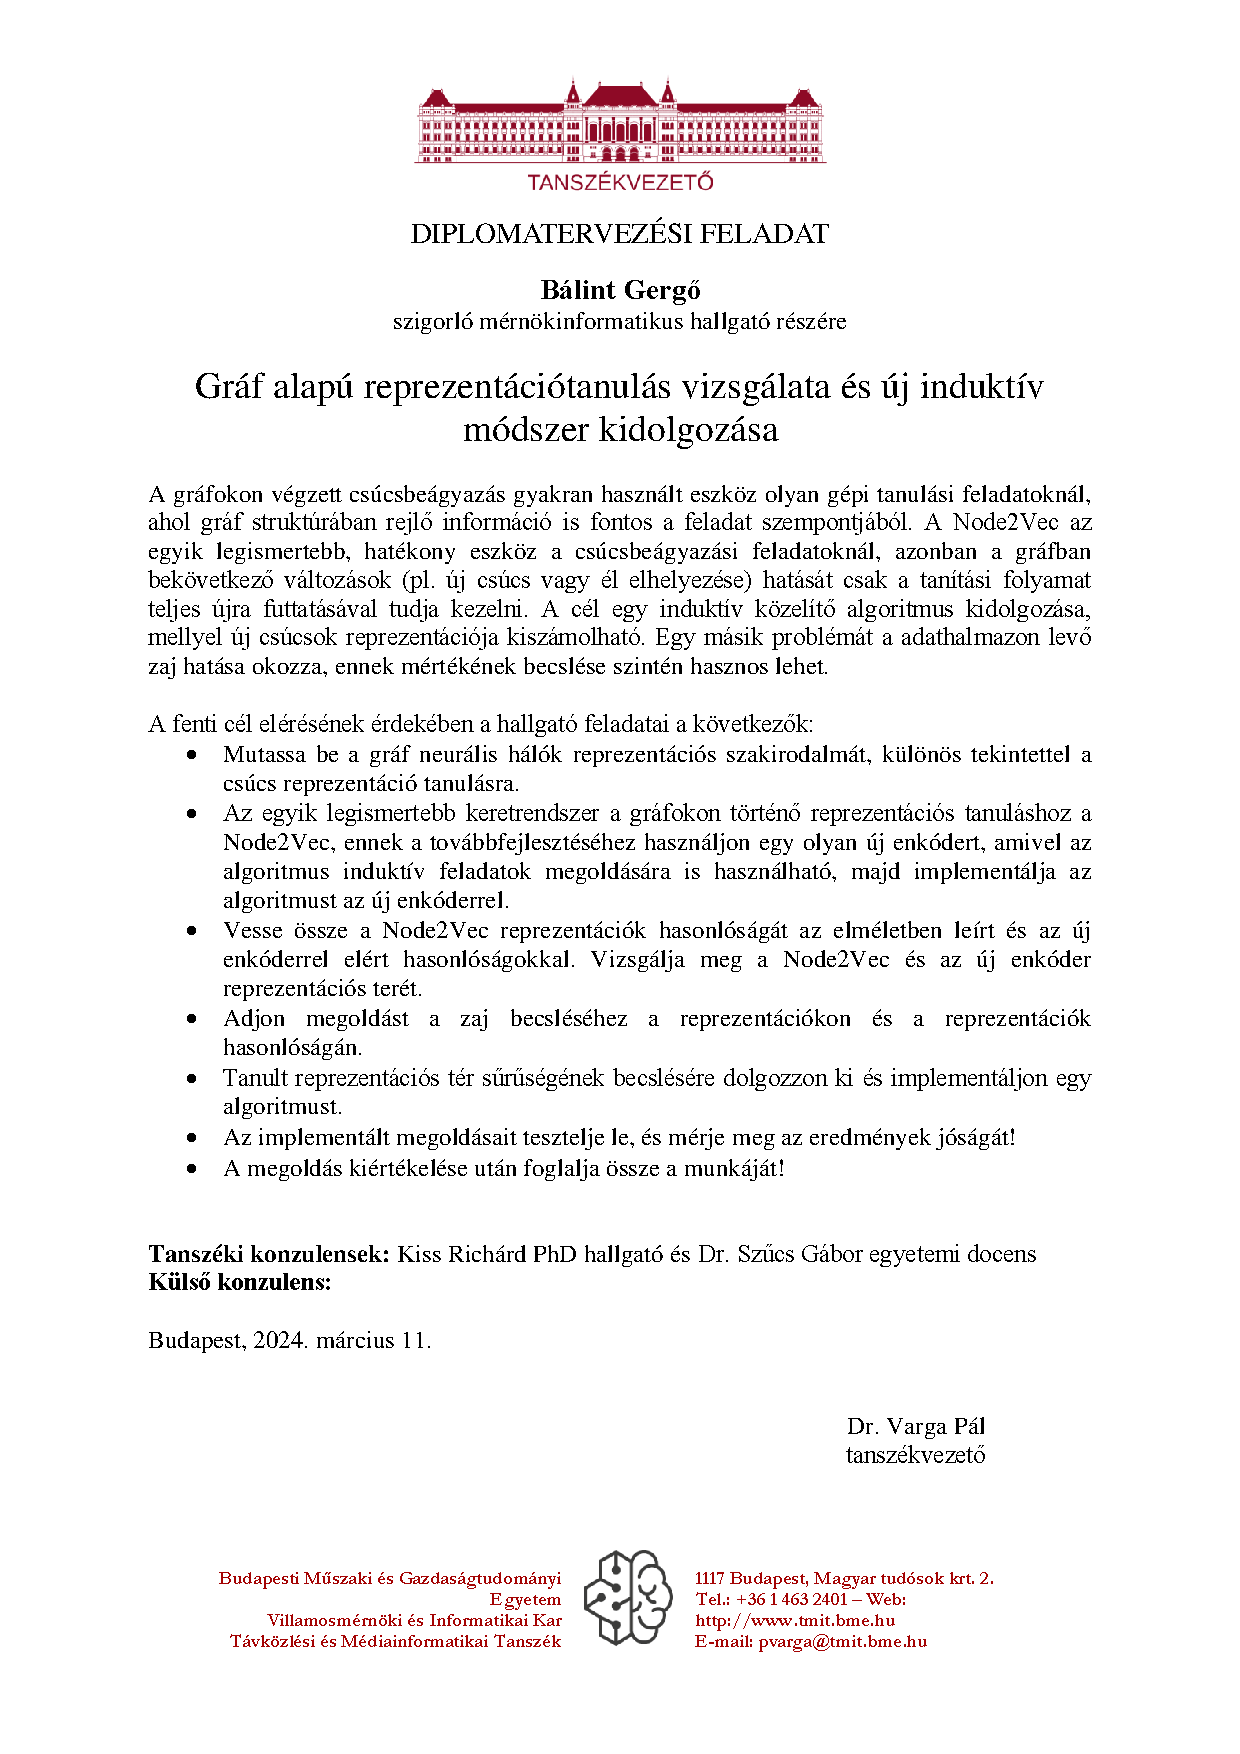
\includepdf[pages=-]{figures/feladatkiiras.pdf}

% Table of Contents
%~~~~~~~~~~~~~~~~~~~~~~~~~~~~~~~~~~~~~~~~~~~~~~~~~~~~~~~~~~~~~~~~~~~~~~~~~~~~~~~~~~~~~~
\tableofcontents\vfill


% Declaration and Abstract
%~~~~~~~~~~~~~~~~~~~~~~~~~~~~~~~~~~~~~~~~~~~~~~~~~~~~~~~~~~~~~~~~~~~~~~~~~~~~~~~~~~~~~~
\selectlanguage{magyar}
\pagenumbering{gobble}
%--------------------------------------------------------------------------------------
% Nyilatkozat
%--------------------------------------------------------------------------------------
\begin{center}
\large
\textbf{HALLGATÓI NYILATKOZAT}\\
\end{center}

Alulírott \emph{\vikszerzoVezeteknev{} \vikszerzoKeresztnev}, szigorló hallgató kijelentem, hogy ezt a \vikmunkatipusat{} meg nem engedett segítség nélkül, saját magam készítettem, csak a megadott forrásokat (szakirodalom, eszközök stb.) használtam fel. Minden olyan részt, melyet szó szerint, vagy azonos értelemben, de átfogalmazva más forrásból átvettem, egyértelműen, a forrás megadásával megjelöltem.

Hozzájárulok, hogy a jelen munkám alapadatait (szerző(k), cím, angol és magyar nyelvű tartalmi kivonat, készítés éve, konzulens(ek) neve) a BME VIK nyilvánosan hozzáférhető elektronikus formában, a munka teljes szövegét pedig az egyetem belső hálózatán keresztül (vagy autentikált felhasználók számára) közzétegye. Kijelentem, hogy a benyújtott munka és annak elektronikus verziója megegyezik. Dékáni engedéllyel titkosított diplomatervek esetén a dolgozat szövege csak 3 év eltelte után válik hozzáférhetővé.

\begin{flushleft}
\vspace*{1cm}
Budapest, \today
\end{flushleft}

\begin{flushright}
 \vspace*{1cm}
 \makebox[7cm]{\rule{6cm}{.4pt}}\\
 \makebox[7cm]{\emph{\vikszerzoVezeteknev{} \vikszerzoKeresztnev}}\\
 \makebox[7cm]{hallgató}
\end{flushright}
\thispagestyle{empty}

\vfill
\clearpage
\thispagestyle{empty} % an empty page

\selectthesislanguage
 %TODO Hallgatói nyilatkozat -- TDK és OTDK esetén törlendő!
\pagenumbering{roman}
\setcounter{page}{1}

\selecthungarian

%----------------------------------------------------------------------------
% Abstract in Hungarian
%----------------------------------------------------------------------------
\chapter*{Kivonat}\addcontentsline{toc}{chapter}{Kivonat}

Jelen dokumentum egy diplomaterv sablon, amely formai keretet ad a BME Villamosmérnöki és Informatikai Karán végző hallgatók által elkészítendő szakdolgozatnak és diplomatervnek. A sablon használata opcionális. Ez a sablon \LaTeX~alapú, a \emph{TeXLive} \TeX-implementációval és a PDF-\LaTeX~fordítóval működőképes.


\vfill
\selectenglish


%----------------------------------------------------------------------------
% Abstract in English
%----------------------------------------------------------------------------
\chapter*{Abstract}\addcontentsline{toc}{chapter}{Abstract}

This document is a \LaTeX-based skeleton for BSc/MSc~theses of students at the Electrical Engineering and Informatics Faculty, Budapest University of Technology and Economics. The usage of this skeleton is optional. It has been tested with the \emph{TeXLive} \TeX~implementation, and it requires the PDF-\LaTeX~compiler.


\vfill
\selectthesislanguage

\newcounter{romanPage}
\setcounter{romanPage}{\value{page}}
\stepcounter{romanPage}    %TODO Összefoglaló -- TDK és OTDK esetén nem kötelező


% The main part of the thesis
%~~~~~~~~~~~~~~~~~~~~~~~~~~~~~~~~~~~~~~~~~~~~~~~~~~~~~~~~~~~~~~~~~~~~~~~~~~~~~~~~~~~~~~
\pagenumbering{arabic}

%TODO import your own content
%----------------------------------------------------------------------------
\chapter{\bevezetes}
%----------------------------------------------------------------------------

Graph-based representation learning has emerged as a cornerstone in the realm of machine learning and artificial intelligence, owing to its ability to effectively capture and interpret complex relationships inherent in graph-structured data. Among these techniques, node2vec stands out for its prowess in generating meaningful node embeddings. However, its applicability to dynamic graphs, where the structure evolves over time, remains a challenge. As such, this thesis is motivated by the imperative to enhance node2vec and similar methods to accommodate dynamic graph changes effectively. By introducing a novel encoder tailored to handle dynamic graph fluctuations, this research aims to advance the capabilities of graph-based representation learning. Such improvements not only address the challenges posed by dynamic graphs but also contribute to the broader objective of developing more robust and adaptable solutions for analyzing and understanding graph-structured data.

This new encoder is referenced Inductive Shallow Node Embedding (ISNE) in the literature, and most of my tasks were to implement it, perform measurements and prepare further research on it.

In this thesis my tasks included presenting the literature on graph neural networks' representation, with particular emphasis on node representation learning. This involved reviewing existing research and summarizing key findings to establish a foundation for further exploration. I present two common methods, DeepWalk and node2vec. The second chapter is dedicated to this.

I was tasked with utilizing a new encoder to further develop node2vec, one of the most well-known frameworks for representation learning on graphs. The objective was to enable the algorithm to solve inductive tasks and improve its overall performance. This required implementing the algorithm with the new encoder, involving coding and refining the implementation to ensure its effectiveness. An important aspect of the project was comparing the similarity of node2vec representations with the similarities achieved theoretically and with the new encoder. This involved conducting quantitative analyses and evaluating the results to assess the efficacy of the new encoder in enhancing representation similarity. The theoretical description of the new encoder, its motivation, and the comparison of the results with the conventional node2vec are discussed in the third chapter.

Furthermore, I was required to provide a solution for noise estimation on the representations and their similarities. This task involved devising algorithms and methodologies to accurately estimate noise levels in the representation space, contributing to the robustness and reliability of the representations. Chapter four provides the background and a description of the results measured.

Additionally, I developed and implemented an algorithm to estimate the density of the learned representation space. This task required designing computational methods and conducting experiments to estimate the density distribution, providing valuable insights into the structure and characteristics of the representation space. The design of the algorithm and the results obtained using it are presented in chapter five. 

I have devoted a separate chapter to examining the explicability of the classifiers learned on the embeddings produced. This is a human-centred AI aspect that is essential because of the spread and new regulation of AI. I discuss this in chapter six.

Finally, I tested and measured the quality of the implemented solutions, assessing their performance and effectiveness. This involved conducting experiments, analyzing results, and identifying areas for improvement to refine the solutions further. After evaluating the solutions and completing the tasks, in chapter seven, I summarized my work, providing a comprehensive overview of the methodologies, findings, and implications of the research conducted throughout the project. 

%----------------------------------------------------------------------------
\chapter{Graph neural networks and representation learning}
\label{sec:RepresentationLearning}
%----------------------------------------------------------------------------

\section{Graph neural networks}
%----------------------------------------------------------------------------

Graph Neural Networks (GNNs) are a class of neural networks designed to process and analyze graph-structured data. Unlike traditional neural networks that operate on Euclidean data such as images and text, GNNs work on data represented as graphs, which can capture complex relationships between entities. The importance of GNNs stems from the ubiquity of graph-structured data in various domains:

\begin{itemize}
    \item \emph{Social Networks:} where nodes represent individuals and edges represent relationships or interactions.
    \item \emph{Biological Networks:} such as protein-protein interaction networks, where nodes represent proteins and edges represent interactions.
    \item \emph{Knowledge Graphs:} where nodes represent entities and edges represent relationships between them.
    \item \emph{Infrastructure Networks:} such as transportation and communication networks.
\end{itemize}

GNNs leverage the graph structure to perform tasks like node classification, link prediction, and graph classification, achieving state-of-the-art performance in many applications.
The field of GNNs has seen rapid growth, driven by advances in machine learning and the increasing availability of graph data. Key milestones in the development of GNNs include the introduction of Graph Convolutional Networks (GCNs), Graph Attention Networks (GATs), and various other architectures that have expanded the capabilities and applications of GNNs.

It is essential to understand the basic components of graph structures. Nodes, or vertices, represent entities within the graph, while edges denote the relationships or connections between these nodes. The adjacency matrix is a square matrix used to represent a graph. In this matrix, the element at row $i$ and column $j$ indicates the presence or weight of an edge between nodes $i$ and $j$. This foundational understanding of graph structures is crucial for comprehending how GNNs operate on graph-structured data.
Graph data presents unique challenges that differ from traditional \verb+Euclidean data+\footnote{
Euclidean data refers to data that exists within the Euclidean space. It is characterized by having a fixed and regular geometric structure. Examples are images, where data points (pixels) are arranged in a regular grid, and each pixel has a fixed position relative to others and tabular data, where entries are organized in rows and columns within a fixed structure.
}. One primary challenge is its non-Euclidean nature, as graphs lack a fixed geometric structure, making it difficult to apply traditional convolutional neural network (CNN) operations. Additionally, graphs exhibit irregularity, where nodes can have varying numbers of neighbors, unlike pixels in an image which have a fixed number of neighboring pixels. Furthermore, the features of a node in a graph depend not only on the node itself but also on its neighbors and their connections, adding a layer of complexity to the learning process.

In Graph Neural Networks, fundamental operations are crucial for processing graph data. Message passing enables nodes to exchange information with their neighbors, involving the aggregation of features and subsequent updates to node representations. Aggregation is then employed to combine neighboring node features through operations like mean, sum, or max. Finally, nodes update their representations based on the aggregated information. These operations, although independent, collectively empower GNNs to effectively analyze and process graph data.

Training approaches for Graph Neural Networks encompass diverse methodologies designed for distinct learning paradigms. \cite{DBLP:journals/corr/abs-1812-08434} In supervised learning, GNNs tackle tasks such as node classification, edge prediction, and graph classification. Node classification involves assigning labels to nodes based on their features and connections within the graph. Edge prediction focuses on predicting the existence or properties of edges between nodes. Graph classification aims to classify entire graphs based on their structural and feature characteristics.

In unsupervised learning, GNNs leverage techniques like graph autoencoders and contrastive learning. Graph autoencoders aim to learn meaningful representations of graphs by reconstructing them from compressed embeddings. Contrastive learning involves training the model to distinguish between positive and negative samples, enhancing its ability to capture meaningful patterns in the data.

Semi-supervised learning techniques in GNNs integrate both labeled and unlabeled data to improve performance. By leveraging a combination of labeled data, where nodes or graphs have known labels, and unlabeled data, where labels are absent, semi-supervised learning enables GNNs to generalize better and make predictions on unseen data. \cite{DBLP:journals/corr/KipfW16} These strategies play a pivotal role in enhancing the adaptability and performance of GNNs across various tasks and datasets.

GNNs have revolutionized the field of graph-based machine learning by enabling effective analysis and processing of complex graph-structured data. One key aspect of these networks is node embedding, a technique that involves representing nodes in a graph as low-dimensional vectors in a continuous vector space. Node embedding is crucial for capturing the structural and semantic relationships between nodes, allowing GNNs to learn meaningful representations of graph elements. By leveraging node embedding, the network can perform various tasks such as node classification, link prediction, and community detection with improved accuracy and efficiency. This capability to encode graph structures into vector representations enables GNNs to generalize to unseen data and handle large-scale graph datasets, making them a powerful tool for tasks ranging from social network analysis to drug discovery and recommendation systems.


\section{Motivation for representation learning}
%----------------------------------------------------------------------------

In the realm of graph-structured data, the motivation for representation learning lies in the extraction of inner representations in a latent space. These representations serve as compact, semantically rich encodings of the underlying graph structure, enabling their utilization as input to various machine learning algorithms. The key motivations for pursuing such representations are as follows: \cite{DBLP:journals/corr/abs-1709-05584}

\begin{itemize}

    \item \emph{Feature Engineering Simplification:} representation learning alleviates the need for manual feature engineering by automatically generating meaningful representations directly from the graph data. This simplification accelerates the model development process and enhances the scalability of graph-based machine learning tasks.

    \item \emph{Enhanced Generalization:} inner representations in a latent space facilitate enhanced generalization of learned patterns and relationships within the graph data. By capturing the essential characteristics of nodes and edges, these representations enable models to make accurate predictions on unseen data and generalize effectively across diverse tasks.

    \item \emph{Interpretability and Visualization:} the learned representations offer insights into the underlying structure of the graph, enhancing interpretability and enabling intuitive visualization of complex relationships between entities. By mapping nodes to points in a low-dimensional latent space, the inner representations reveal clusters, communities, and structural similarities within the graph.

    \item \emph{Integration with Machine Learning Algorithms:} the compact nature of inner representations makes them ideal inputs for various machine learning algorithms. Whether for classification, regression, or clustering tasks, these representations provide a concise yet informative representation of the graph data, facilitating seamless integration with existing machine learning pipelines.

    \item \emph{Scalability and Efficiency:} representation learning techniques often exhibit scalability and computational efficiency, enabling the analysis of large-scale graph datasets in real-time or near real-time. This scalability is essential for applications across diverse domains, from social network analysis to recommendation systems and beyond.

\end{itemize}

In essence, the motivation for representation learning in the context of graph-structured data centers on the extraction of inner representations in a latent space. When learning representation, an important goal is to produce tabular, low-dimensional embeddings that allow us to infer the structure of the original graph without losing information about it. There are several known methods and algorithms for learning latent representations, two of the most common of which, DeepWalk and Node2Vec, are discussed in this thesis.

\section{DeepWalk} 
%----------------------------------------------------------------------------
TODO [1.5 oldal]

cikk és előadásom alapján

\section{Node2Vec algorithm}
%----------------------------------------------------------------------------
TODO [2.5 oldal]

cikk és előadásom alapján

+ pseudo algorithm
%----------------------------------------------------------------------------
\chapter{Inductive Shallow Node Embedding}
\label{sec:ISNE}
%----------------------------------------------------------------------------

\section{Problems with shallow encoders}
%----------------------------------------------------------------------------
In the previous chapter I presented the DeepWalk and node2vec algorithms for computing graph embeddings. They are both traditional shallow embedding methods, which rely on a lookup table encoder architecture.

Shallow Encoder Algorithms initially use a lookup table to represent nodes, where each node is assigned a unique embedding vector pre-defined in a low-dimensional space. This process, represented by the function $f$, essentially maps each node $v$ in the network to its corresponding embedding vector: ${f(v) = \Theta v}$.

However, algorithms employing lookup table encoders face two significant limitations:

\begin{enumerate}

    \item \emph{Transductivity:} node2vec and similar methods relying on lookup tables are inherently transductive. This means they cannot effectively generalize to unseen nodes that were not part of the training data. Consequently, their utility is restricted in scenarios involving dynamic networks or tasks necessitating predictions for new nodes.

    \item \emph{Static Embeddings:} the embeddings produced by node2vec are static; they do not dynamically update in response to changes in the network structure, such as edge additions or removals. This lack of adaptability poses challenges in real-world networks that frequently undergo dynamic alterations.

\end{enumerate}

These limitations make shallow embedding techniques unsuitable for tasks on continuously changing graphs, as even small changes in the graph can degrade the performance of the model significantly, and after more changes the model can easily become unusable. The static model cannot predict anything about new nodes. 

My task in this thesis is to implement a new dynamic encoder and compare it with the traditional encoder on different graph datasets by taking measurements. 

\section{Inductive Shallow Node Embedding}
%----------------------------------------------------------------------------

Inductive Shallow Node Embedding (ISNE) is a new dynamic graph embedding method proposed by $Richárd Kiss$ and $Gábor Szűcs$ in their paper [TODO cite]. ISNE employs an innovative encoder function designed to overcome the obstacles posed by both previously unseen nodes and dynamic network structures. This sophisticated design enables ISNE to:

\begin{itemize}
    \item \emph{Generalize to Unseen Nodes:} unlike transductive methodologies, ISNE is capable of effectively representing nodes that were not present during the training phase.
    \item \emph{Adapt to Dynamic Networks:} ISNE's representations can seamlessly adjust to modifications in the network structure, rendering them suitable for networks that evolve over time.
    \item \emph{Operate Independently of Node Attributes:} ISNE constructs embeddings exclusively based on the network's structure, thereby obviating the dependency on potentially unreliable or unavailable node attribute information.
\end{itemize}

Moreover, ISNE maintains the adaptability to incorporate node attributes by concatenating them to the existing ISNE embeddings. This feature allows users to harness the advantages of both network structure and node attributes, potentially yielding more robust and informative representations. Contrary to conventional shallow embedding techniques that rely on lookup tables, the proposed Inductive Shallow Node Embedding (ISNE) method utilizes a novel encoder function to construct node embeddings. This function operates based on the immediate neighbors of each node, as represented by the neighborhood set $N_v$. The fundamental update-step for the ISNE encoder is expressed in Equation~\ref{neigborhood}.

\clearpage

In this equation, ${h(v)}$ denotes the embedding vector of node 
$v$, with the summation iterating through all neighbors 
$n$ within its neighborhood set. This design ensures that a node's embedding is informed by the parameters of its immediate neighbors, effectively capturing the local network structure surrounding each node.

\begin{equation}
\label{neigborhood}
h(v) = \frac{1}{|N_v|} \sum_{n \in N_v} \theta_n
\end{equation}

This approach offers several critical advantages. Whenever a new edge is introduced to the network, the neighborhood set of the affected nodes (i.e., $N_j$ for specific nodes 
$j$) is updated accordingly. By recalculating ${h(v)}$ for these nodes, ISNE embeddings inherently reflect the latest structural changes within their local neighborhoods. The ISNE framework can generate embeddings for nodes that were previously unseen, provided their connections are known. By incorporating these connections into the neighborhood set during the encoding process (i.e., adding them to $N_v$ for the unseen node), ISNE can effectively estimate their embeddings.

This unique design also enables ISNE to perform inductive learning tasks. By relying solely on the network's structure and generalizing from existing information, the model can infer embeddings for unseen and modified data points, significantly enhancing its applicability in dynamic network settings and demonstrating adaptability to evolving graph structures.

In essence, the ISNE encoder transcends the limitations of traditional lookup tables by facilitating dynamic updates, accommodating unseen nodes, and supporting inductive learning tasks, thereby establishing itself as a critical tool for various network analysis applications.

\section{Comparison of different encoder result representations and theoretical representations}
%----------------------------------------------------------------------------

My task was to implement the new encoder (ISNE) and the node2vec algorithm, and then to train and evaluate the resulting models with different parameterizations on several data sets. I did a triple comparison, since I had to compare the similarity matrix derived from the embeddings of the two models with an implicit approximated and computed matrix. \cite{DBLP:journals/corr/abs-1710-02971} \cite{DBLP:journals/corr/YangL15} This matrices can be calculated both for DeepWalk and node2vec, using only the properties of the input graph and the hyperparameters used to teach it, as seen for DeepWalk in Equation~\ref{dw_M} and for node2vec Equation~\ref{n2v_M}

\begin{align}
\label{dw_M}
\log \left( {\text{vol}(G)} \left( \frac{1}{T} \sum_{r=1}^{T} \left( D^{-1}A \right)^r \right) D^{-1} \right) - \log b
\end{align}

\begin{align}
\label{n2v_M}
\log \left( \frac{1}{2T} \sum_{r=1}^{T} \left( \frac{\sum_{u} X_{w,u} P^{r}_{c,w,u} + \sum_{u} X_{c,u} P^{r}_{w,c,u}}{(\sum_{u} X_{w,u})(\sum_{u} X_{c,u})} \right) \right) - \log b
\end{align}

In the equations the following declarations were used \cite{DBLP:journals/corr/abs-1710-02971} \cite{DBLP:journals/corr/YangL15}:

\begin{itemize}
    \item \textbf{A:} $A \in \mathbb{R}_{+}^{|V| \times |V|}$ is $G$'s adjacency matrix with $A_{i,j}$ as the edge weight between vertices $i$ and $j$;
    \item \textbf{D\textsubscript{col}:} $D_{\text{col}} = \text{diag}(A^T e)$ is the diagonal matrix with the column sum of $A$;
    \item \textbf{D\textsubscript{row}:} $D_{\text{row}} = \text{diag}(Ae)$ is the diagonal matrix with the row sum of $A$;
    \item \textbf{D:} For undirected graphs $(A^T = A)$, $D_{\text{col}} = D_{\text{row}}$. For brevity, $D$ represents both $D_{\text{col}}$ and $D_{\text{row}}$. $D = \text{diag}(d_1, \ldots, d_{|V|})$, where $d_i$ represents the generalized degree of vertex $i$;
    \item \textbf{vol(G):} $\text{vol}(G) = \sum_{i} \sum_{j} A_{i,j} = \sum_{i} d_i$ is the volume of a weighted graph $G$;
    \item \textbf{T \& b:} The context window size and the number of negative sampling in skip-gram, respectively.
\end{itemize}

After calculating the implicit approximation of the matrices, I first compared the embeddings of node2vec using the traditional node2vec and the new decoder (ISNE). From the embeddings we can derive the similarity matrix interpreted on the vertices by taking the dot product of the embeddings with their transposed form. To calculate the similarity of the matrices, I used the following metrics:

\begin{enumerate}
    \item Using the Flatten function, I can get one-dimensional lists from the matrices, and plot two lists as a pair of points. Looking at this epoch by epoch, you can see that these points converge to the vicinity of the ${x=y}$ line. The closer they are to this line, the more similar the two similarity matrices, and hence the more similar the learned latent representations. Due to the large number of point pairs and their close proximity, I decided to use a heatmap to represent this.

    \item As in the previous point, the correlation coefficient between the two lists can be calculated. By calculating this for each epoch, we can plot the evolution of this coefficient during learning, ideally increasing it, since we expect that if we learn to convergence, the embeddings of the two models will be highly correlated.
\end{enumerate}

These methods can be used to show the degree of similarity of the matrices when comparing the three matrix sources. The measurements were made on several different sets of graph data, and with different hyperparameters during the training, which were naturally the same in the two models in a single measurement. Below are some visual results as examples, further results are detailed in the Appendix. Result of my first method shown on Figure~\ref{start_hm} and Figure~\ref{result_hm}. Figure~\ref{coef_res} displays the result of my second  method.

\begin{figure}[ht!]
	\centering
	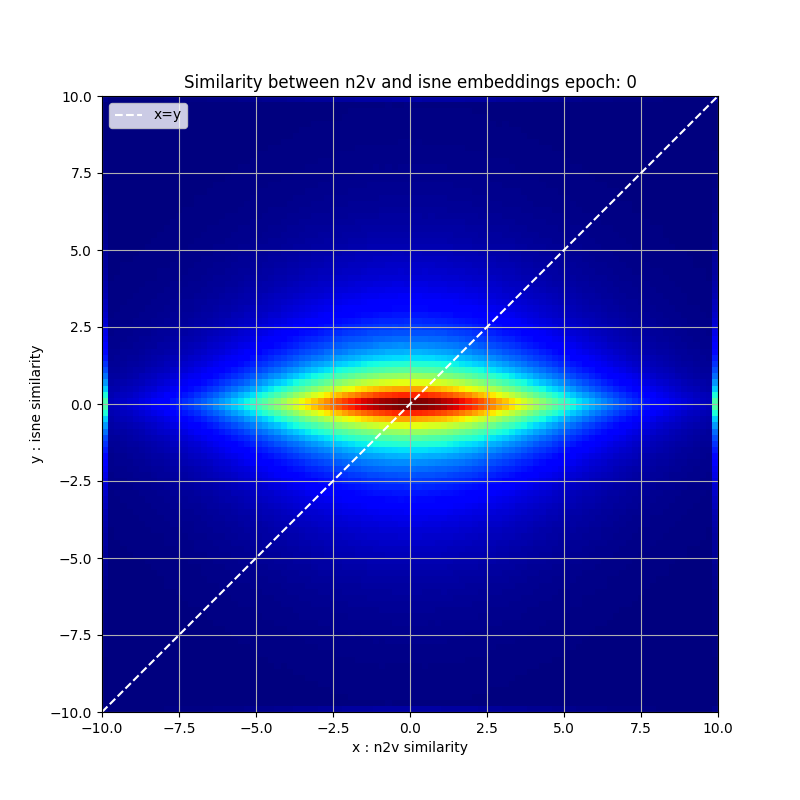
\includegraphics[width=0.70\textwidth]{figures/start_hm.png}
	\caption{On PubMed dataset, with ${p = 0.5, q =0.5}$ hiperparameters, initialization step, normalized noise.}
	\label{start_hm}
\end{figure}

\begin{figure}[ht!]
	\centering
	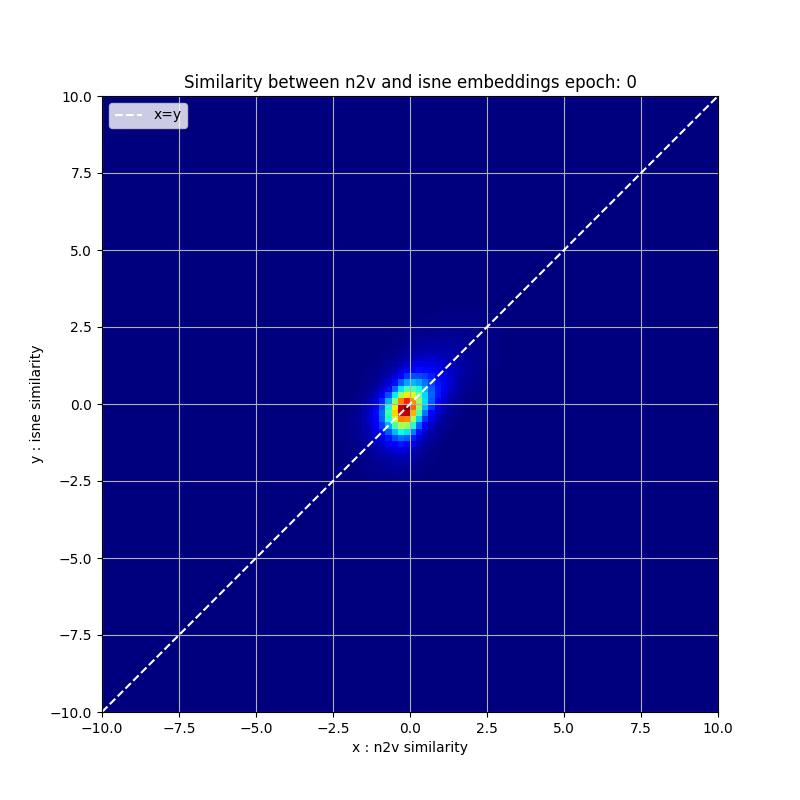
\includegraphics[width=0.70\textwidth]{figures/result_hm.png}
	\caption{On PubMed dataset, with ${p = 0.5, q =0.5}$ hiperparameters, after 40. epoch.}
	\label{result_hm}
\end{figure}

\begin{figure}[ht!]
	\centering
	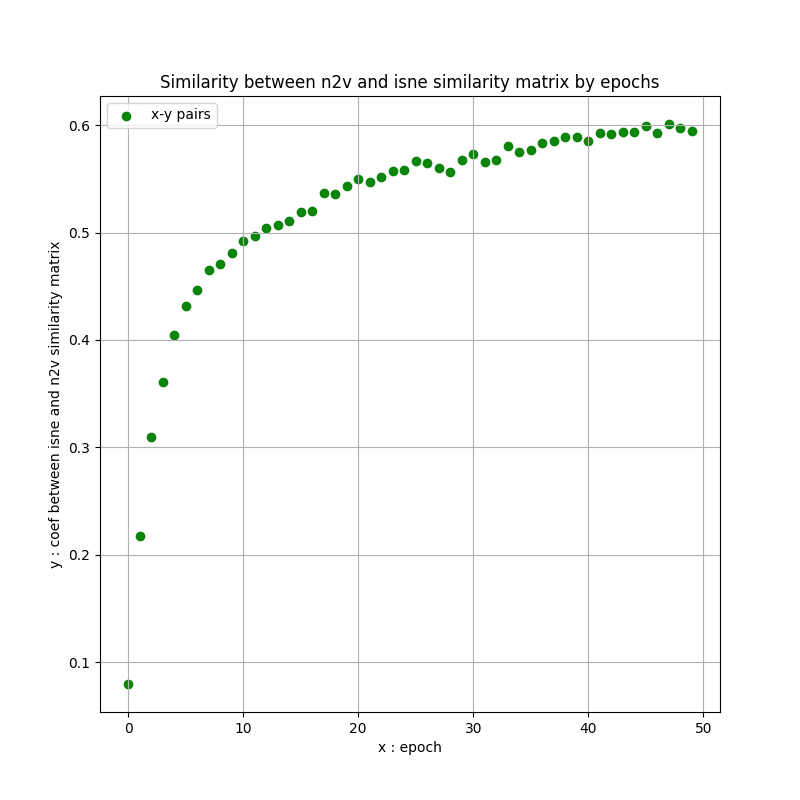
\includegraphics[width=0.70\textwidth]{figures/Cora_05_05_coef_plot.png}
	\caption{On PubMed dataset, with ${p = 0.5, q =0.5}$ hiperparameters, correlation coef through 50 epoch.}
	\label{coef_res}
\end{figure}
%----------------------------------------------------------------------------
\chapter{Noise estimation on embedded representations}
\label{sec:Noise}
%----------------------------------------------------------------------------

\section{Theoretical background to noise estimation}
%----------------------------------------------------------------------------
TODO


\section{Comparison of estimated noise on the results of different methods}
%----------------------------------------------------------------------------
TODO
%----------------------------------------------------------------------------
\chapter{Density estimation of the learned representational space}
\label{sec:Density}
%----------------------------------------------------------------------------

\section{Algorithm design for density estimation}
%----------------------------------------------------------------------------
TODO


\section{Density analysis of the learned representational space}
%----------------------------------------------------------------------------
TODO

%----------------------------------------------------------------------------
\chapter{Examining explainability on classifiers using learned representations}
\label{sec:Explainability}
%----------------------------------------------------------------------------

\section{HCAIM aspects}
%----------------------------------------------------------------------------
TODO

\section{Classification tasks on graphs}
%----------------------------------------------------------------------------
TODO

%----------------------------------------------------------------------------
\chapter{Measurement results and summary}
\label{sec:Summary}
%----------------------------------------------------------------------------

\section{Summary of the thesis}
%----------------------------------------------------------------------------
TODO

\section{Measurement results}
%----------------------------------------------------------------------------
TODO


% Acknowledgements
%~~~~~~~~~~~~~~~~~~~~~~~~~~~~~~~~~~~~~~~~~~~~~~~~~~~~~~~~~~~~~~~~~~~~~~~~~~~~~~~~~~~~~~
%%----------------------------------------------------------------------------
\chapter*{\koszonetnyilvanitas}\addcontentsline{toc}{chapter}{\koszonetnyilvanitas}
%----------------------------------------------------------------------------

Ez nem kötelező, akár törölhető is. Ha a szerző szükségét érzi, itt lehet köszönetet nyilvánítani azoknak, akik hozzájárultak munkájukkal ahhoz, hogy a hallgató a szakdolgozatban vagy diplomamunkában leírt feladatokat sikeresen elvégezze. A konzulensnek való köszönetnyilvánítás sem kötelező, a konzulensnek hivatalosan is dolga, hogy a hallgatót konzultálja.


% List of Figures, Tables
%~~~~~~~~~~~~~~~~~~~~~~~~~~~~~~~~~~~~~~~~~~~~~~~~~~~~~~~~~~~~~~~~~~~~~~~~~~~~~~~~~~~~~~
%\listoffigures\addcontentsline{toc}{chapter}{\listfigurename}
%\listoftables\addcontentsline{toc}{chapter}{\listtablename}


% Bibliography
%~~~~~~~~~~~~~~~~~~~~~~~~~~~~~~~~~~~~~~~~~~~~~~~~~~~~~~~~~~~~~~~~~~~~~~~~~~~~~~~~~~~~~~
\addcontentsline{toc}{chapter}{\bibname}
\bibliography{bib/mybib}


% Appendix
%~~~~~~~~~~~~~~~~~~~~~~~~~~~~~~~~~~~~~~~~~~~~~~~~~~~~~~~~~~~~~~~~~~~~~~~~~~~~~~~~~~~~~~
%----------------------------------------------------------------------------
\appendix
%----------------------------------------------------------------------------
\chapter*{\fuggelek}\addcontentsline{toc}{chapter}{\fuggelek}
\setcounter{chapter}{\appendixnumber}
%\setcounter{equation}{0} % a fofejezet-szamlalo az angol ABC 6. betuje (F) lesz
\numberwithin{equation}{section}
\numberwithin{figure}{section}
\numberwithin{lstlisting}{section}
%\numberwithin{tabular}{section}

%----------------------------------------------------------------------------
\section{A TeXstudio felülete}
%----------------------------------------------------------------------------
\begin{figure}[!ht]
\centering
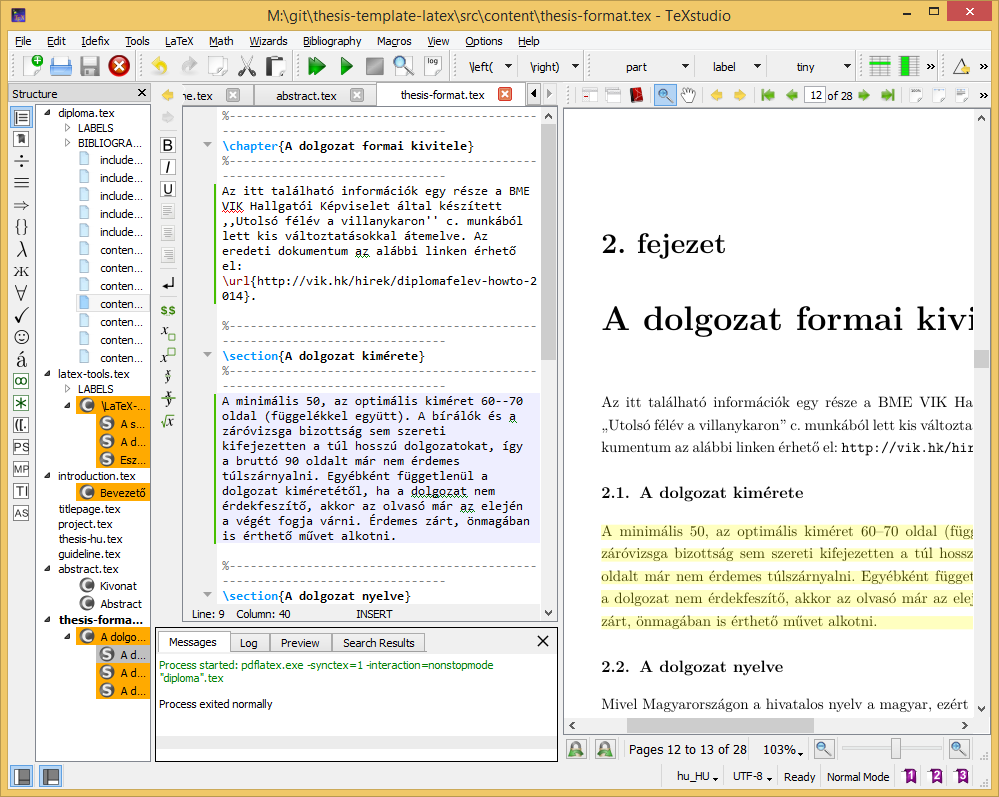
\includegraphics[width=150mm, keepaspectratio]{figures/TeXstudio.png}
\caption{A TeXstudio \LaTeX-szerkesztő.} 
\end{figure}

%----------------------------------------------------------------------------
\clearpage\section{Válasz az ,,Élet, a világmindenség, meg minden'' kérdésére}
%----------------------------------------------------------------------------
A Pitagorasz-tételből levezetve
\begin{align}
c^2=a^2+b^2=42.
\end{align}
A Faraday-indukciós törvényből levezetve
\begin{align}
\rot E=-\frac{dB}{dt}\hspace{1cm}\longrightarrow \hspace{1cm}
U_i=\oint\limits_\mathbf{L}{\mathbf{E}\mathbf{dl}}=-\frac{d}{dt}\int\limits_A{\mathbf{B}\mathbf{da}}=42.
\end{align}


%\label{page:last}
\end{document}
